\documentclass{beamer}
\usepackage{caption}
\usepackage{subcaption}
\usetheme{Berkeley}

\begin{document}

\begin{frame}

\begin{figure}
\setcounter{subfigure}{0}. 
	\begin{subfigure}[b]{.4\linewidth}
		\centering
		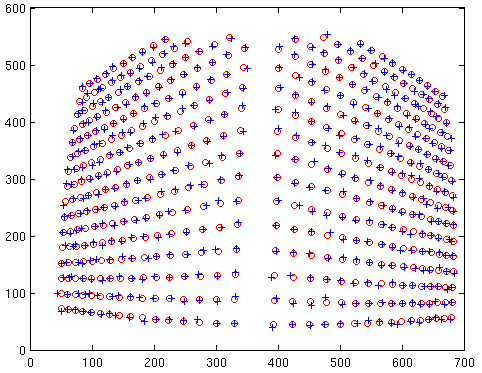
\includegraphics[width=.9\textwidth]{perturb_train}
		\caption{3D Scene}
	\end{subfigure}
	\begin{subfigure}[b]{.5\linewidth}
		\centering
		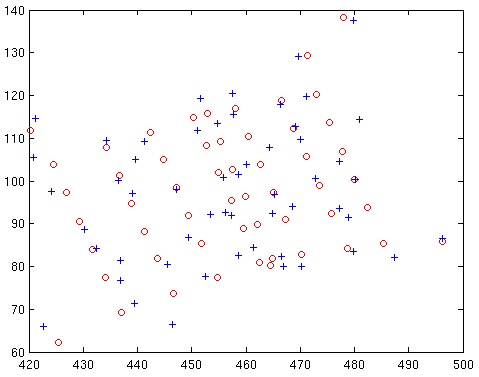
\includegraphics[width=.9\textwidth]{perturb_test}
		\caption{Image of the Scene}
	\end{subfigure}
\end{figure}
\end{frame}


\begin{frame}
\frametitle{Projection Error Vs. Perturbation}
\begin{figure}[H]
\setcounter{subfigure}{0}. 
	\begin{subfigure}[b]{.35\linewidth}
		\centering		
		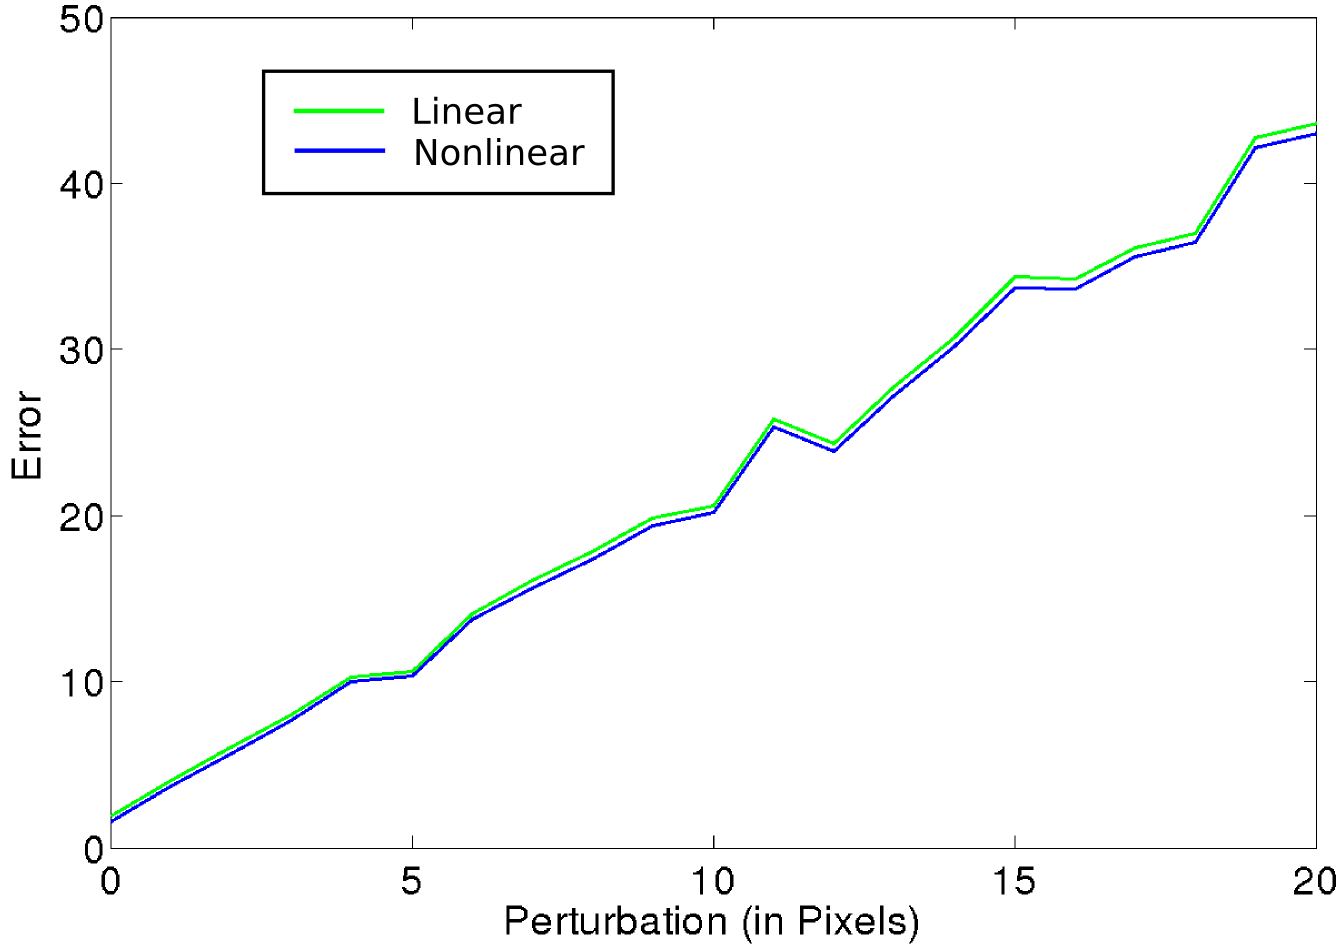
\includegraphics[width=.9\textwidth]{p_err_plot_pert_train}
	 	\caption{Training Data}
	\end{subfigure}

	\begin{subfigure}[b]{.35\linewidth}
		\centering
		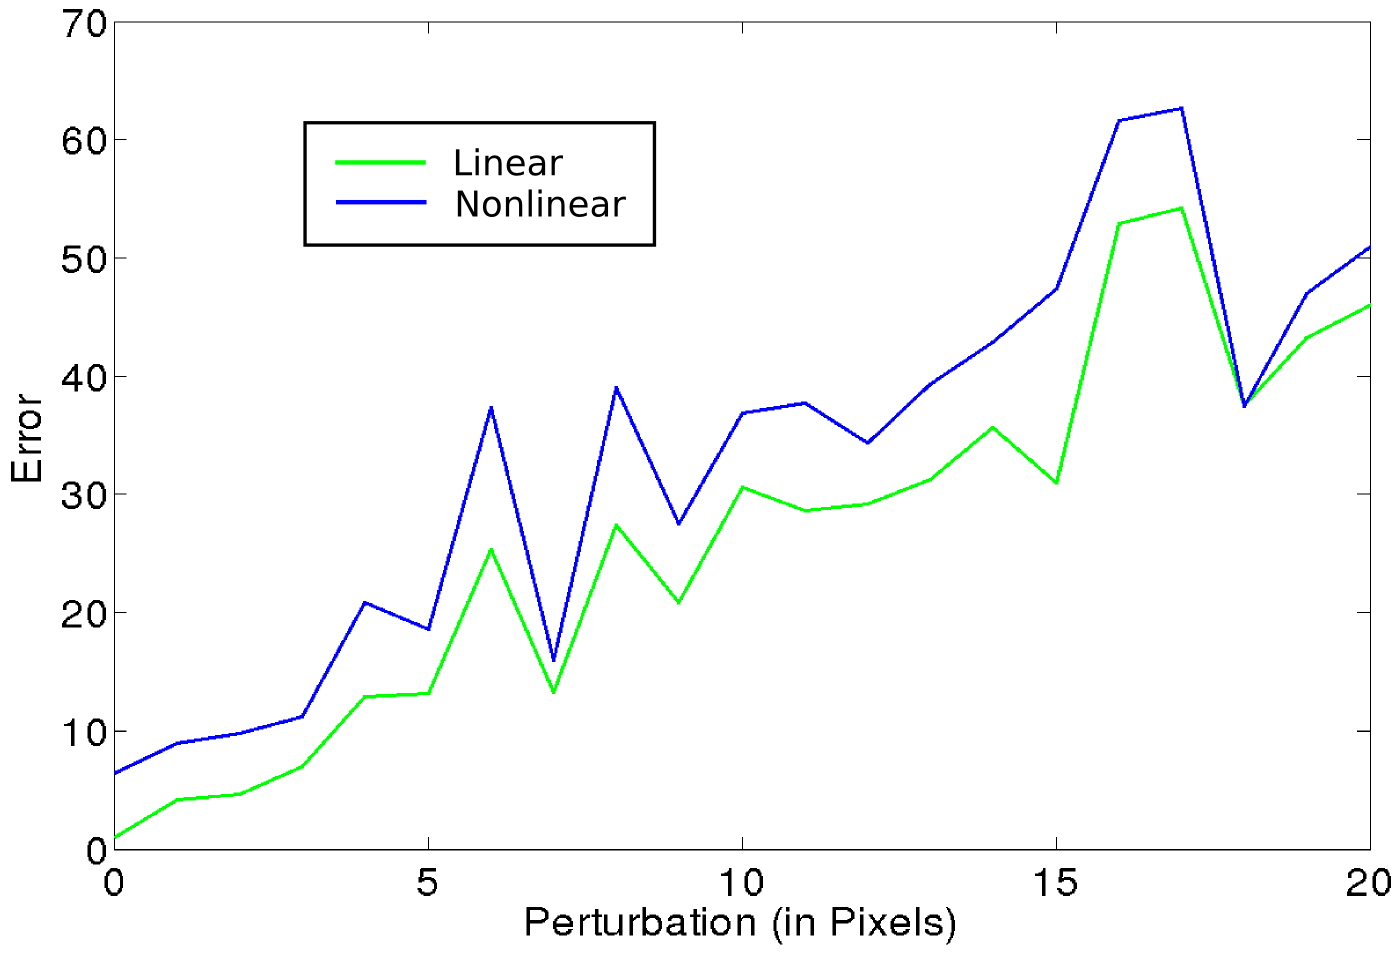
\includegraphics[width=.9\textwidth]{p_err_plot_pert_test}
	 	\caption{Testing Data}
	\end{subfigure}

\end{figure}


\begin{itemize}
\item Poor job accounting for noise
\item Nonlinear method has \textit{more} error
\end{itemize}

\end{frame}

\end{document} 